\renewcommand*{\arraystretch}{1.1}

\subsection*{BI / read / 7}
\label{section:bi-read-07}

% change \emph{} to use sans-serif font
\let\oldemph\emph
\renewcommand{\emph}[1]{{\footnotesize \sf #1}}

\renewcommand{\currentQueryCard}{7}
\marginpar{
	\raggedleft
	\vspace{0.22ex}

	\queryRefCard{bi-read-01}{BI}{1}\\
	\queryRefCard{bi-read-02}{BI}{2}\\
	\queryRefCard{bi-read-03}{BI}{3}\\
	\queryRefCard{bi-read-04}{BI}{4}\\
	\queryRefCard{bi-read-05}{BI}{5}\\
	\queryRefCard{bi-read-06}{BI}{6}\\
	\queryRefCard{bi-read-07}{BI}{7}\\
	\queryRefCard{bi-read-08}{BI}{8}\\
	\queryRefCard{bi-read-09}{BI}{9}\\
	\queryRefCard{bi-read-10}{BI}{10}\\
	\queryRefCard{bi-read-11}{BI}{11}\\
	\queryRefCard{bi-read-12}{BI}{12}\\
	\queryRefCard{bi-read-13}{BI}{13}\\
	\queryRefCard{bi-read-14}{BI}{14}\\
	\queryRefCard{bi-read-15}{BI}{15}\\
	\queryRefCard{bi-read-16}{BI}{16}\\
	\queryRefCard{bi-read-17}{BI}{17}\\
	\queryRefCard{bi-read-18}{BI}{18}\\
	\queryRefCard{bi-read-19}{BI}{19}\\
	\queryRefCard{bi-read-20}{BI}{20}\\
	\queryRefCard{bi-read-21}{BI}{21}\\
	\queryRefCard{bi-read-22}{BI}{22}\\
	\queryRefCard{bi-read-23}{BI}{23}\\
	\queryRefCard{bi-read-24}{BI}{24}\\
	\queryRefCard{bi-read-25}{BI}{25}\\
}


\noindent\begin{tabularx}{\queryCardWidth}{|>{\queryPropertyCell}p{\queryPropertyCellWidth}|X|}
	\hline
	query & BI / read / 7 \\ \hline
%
	title & Most authoritative users on a given topic \\ \hline
%
	pattern & \multicolumn{1}{c|}{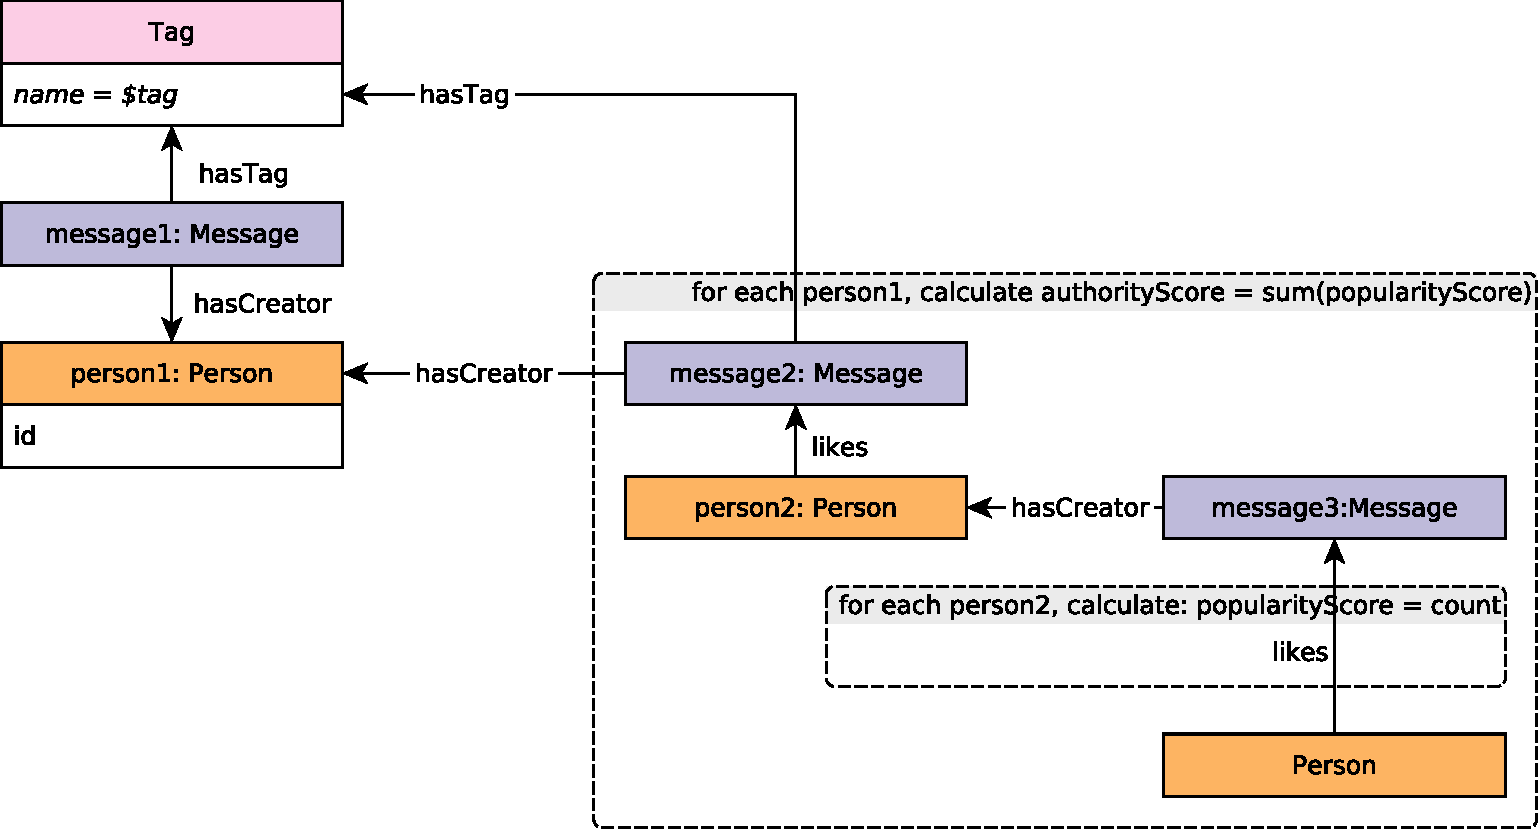
\includegraphics[scale=\patternscale,margin=0cm .2cm]{patterns/bi-read-07}} \\ \hline
%
	desc. & Given a \emph{Tag}, find all \emph{Persons} (\texttt{person}) that ever
created a \emph{Message} (\texttt{message1}) with the given \emph{Tag}.
For each of these \emph{Persons} (\texttt{person}) compute their
``authority score'' as follows:

\begin{itemize}
\tightlist
\item
  The ``authority score'' is the sum of ``popularity scores'' of the
  \emph{Persons} (\texttt{person2}) that liked any of that
  \emph{Person}'s \emph{Messages} (\texttt{message2}) with the given
  \emph{Tag}.
\item
  A \emph{Person}'s (\texttt{person2}) ``popularity score'' is defined
  as the total number of likes on all of their \emph{Messages}
  (\texttt{message3}).
\end{itemize}
 \\ \hline
%
	
		params &
		\innerCardVSpace{\begin{tabularx}{\attributeCardWidth}{|>{\paramNumberCell}c|>{\varNameCell}M|>{\typeCell}m{\typeWidth}|Y|} \hline
		$\mathsf{1}$ & tag
 & String
 &  \\ \hline
		\end{tabularx}}\innerCardVSpace \\ \hline
	
%
	
		result &
		\innerCardVSpace{\begin{tabularx}{\attributeCardWidth}{|>{\resultNumberCell}c|>{\varNameCell}M|>{\typeCell}m{\typeWidth}|>{\resultOriginCell}c|Y|} \hline
		$\mathsf{1}$ & person.id & 64-bit Integer & R &
				 \\ \hline
		$\mathsf{2}$ & authorityScore & 32-bit Integer & A &
				 \\ \hline
		\end{tabularx}}\innerCardVSpace \\ \hline
	
%
	
		sort		&
		\innerCardVSpace{\begin{tabularx}{\attributeCardWidth}{|>{\sortNumberCell}c|>{\varNameCell}M|>{\directionCell}c|Y|} \hline
		$\mathsf{1}$ & authorityScore
 & $\desc
$ &  \\ \hline
		$\mathsf{2}$ & person1.id
 & $\asc
$ &  \\ \hline
		\end{tabularx}}\innerCardVSpace \\ \hline
	%
	limit & 100 \\ \hline
	%
	CPs &
	\multicolumn{1}{>{\raggedright}l|}{
		\chokePoint{1.2}, 
		\chokePoint{2.3}, 
		\chokePoint{3.2}, 
		\chokePoint{3.3}, 
		\chokePoint{6.1}
		} \\ \hline
	%
	%
\end{tabularx}
\queryCardVSpace

% change \emph back to the old one
\renewcommand{\emph}[1]{\oldemph{#1}}